\documentclass[12pt]{article}
\usepackage{pgfplots}
\begin{document}
\title{Statistics 12, Homework 1}
\date{January 20th, 2019}
\author{Michael Wu\\UID: 404751542}
\maketitle

\section*{Chapter 1, Problem 2}

Amazon hopes to gain insight into the customer's buying patterns and interests in order to sell what the people want.
They can also use the data for data mining in order to provide recommendations to customers. This improves the
overall shopping experience for customers and is part of the reason why Amazon is one of the most valuable companies
in the world today.

\section*{Chapter 1, Problem 10}

The researcher is studying a numerical or quantitative variable, as the measured value can be expressed as a
real number of beats per minute.

\section*{Chapter 1, Problem 16}

The other companies are the ``Who'' in this example. The ``What'' that was investigated was the employee 401(k) participation
rates associated with each company. The Population of Interest consists of companies with 401(k) retirement plans
for its employees.

\section*{Chapter 1, Problem 30}

The ``Who'' in this example consists of the car types that were investigated. The ``What'' is the car's information
such as the manufacturer, vehicle type, weight, horsepower, and gas mileage for city and highway
driving. We do not know the ``When'' or the ``Where'' associated with the data collected. The ``Why'' associated with
the data is presumably to monitor the fuel efficiency of each vehicle since more fuel efficient cars are better for
the environment. The variables that are collected are, once again, the manufacturer, vehicle type, weight, horsepower, gas
mileage for city driving, and gas mileage for highway driving. The manufacturer is a categorical variable. The vehicle type
is a categorical variable. The weight is a quantitative variable, though the unit of measurement was not provided. It could
be measured in kilograms or pounds. The horsepower is a quantitative variable, measured in units of horsepower. The gas mileage
for city driving is a quantitative variable, measured in miles per gallon. The gas mileage for highway driving is a quantitative
variable, measured in miles per gallon.

\section*{Chapter 2, Problem 2}

\begin{center}
    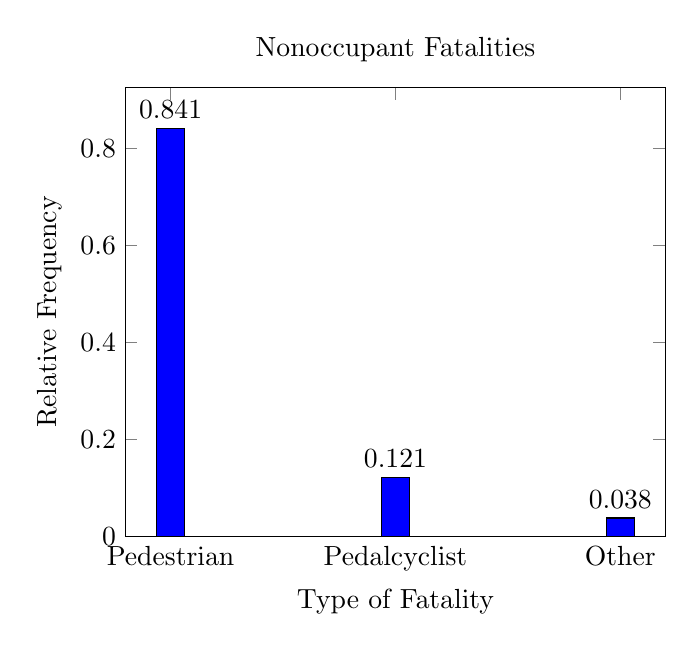
\begin{tikzpicture}
        \begin{axis}[
            symbolic x coords={Pedestrian, Pedalcyclist, Other},
            xtick=data,
            xlabel=Type of Fatality,
            ylabel=Relative Frequency,
            ymin=0,
            title=Nonoccupant Fatalities,
            nodes near coords,
            nodes near coords style={/pgf/number format/.cd,fixed,precision=3}
          ]
            \addplot[ybar, fill=blue] coordinates {
                (Pedestrian, 0.8414657)
                (Pedalcyclist, 0.1209417)
                (Other, 0.03759256)
            };
        \end{axis}
    \end{tikzpicture}
\end{center}

\section*{Chapter 2, Problem 4}

Bar chart i matches with pie chart D. Bar chart ii matches with pie chart A. Bar chart iii matches with pie chart C. Bar chart iv matches with pie chart B.

\section*{Chapter 2, Problem 6}

\paragraph{a)}

6.233\% of those surveyed were unemployed.

\paragraph{b)}

3.725\% of those surveyed were unemployed and aged 25 to 54 years.

\paragraph{c)}

11.066\% of 20 to 24 year olds were unemployed.

\paragraph{d)}

3.148\% of those employed were aged 16 to 19 years.

\section*{Chapter 2, Problem 14}

\paragraph{a)}

G was the least common rating.

\paragraph{b)}

This bar chart does not support this claim. The relative frequencies of G and PG-13 movies are almost the same. The most
noticeable difference is the increase in R rated movies from about 10\% to 30\% of the top movies. So the writer should
have written that the growth in R rated films has come at the expense of G and PG rated films.

\section*{Chapter 2, Problem 16}

The Houston magnet schools program had 29.46\% hispanic, 16.64\% asian, and 53.9\% white applicants.

\section*{Chapter 2, Problem 28}

\paragraph{a)}

82.46\% of seniors are white.

\paragraph{b)}

12.29\% of seniors are planning to attend a 2-year college.

\paragraph{c)}

11.08\% of seniors are white and planning to attend a 2-year college.

\paragraph{d)}

13.43\% of white seniors are planning to attend a 2-year college.

\paragraph{e)}

85.71\% of seniors planning to attend a 2-year college are white.

\end{document}